\appendix

\chapter{Raw JSON Data}

\section{Vignetting Analysis}
\label{app:vignetting_json}
\begin{minted}[linenos, fontsize=\small, breaklines=true]{js}
{
  "id": "g_20241215_130205",
  "name": "g",
  "created": "20241215_130205",
  "metadata": {},
  "scenarios": [
    {
      "id": "vignette_20241215_130554",
      "type": "vignette",
      "created": "20241215_130554",
      "metadata": {
        "focal_length": 50,
        "notes": "",
        "created": "20241215_130554"
      },
      "photos": [
        {
          "filename": "vignette_20241215_132956_2J9B3461.CR2",
          "path": "datasets/g_20...<full path  omitted>",
          "timestamp": "20241215_132956",
          "metadata": {
            "scenario_type": "vignette",
            "scenario_id": "vignette_20241215_130554",
            "camera_settings": {
              "aperture": "2.5",
              "iso": "Auto",
              "shutter_speed": "1/50",
              "camera_model": "Canon EOS 5D Mark III",
              "lens_name": "EF50mm f/2.5 Compact Macro"
            },
            "aperture": "2.5",
            "shutter_speed": "1/50",
            "iso": "Auto",
            "lens_name": "EF50mm f/2.5 Compact Macro",
            "camera_model": "Canon EOS 5D Mark III",
            "focal_length": null
          },
          "analysis": {
            "vignetting_results": {
              "center_intensity": 68.26437152181892,
              "corner_intensities": {
                "top_left": 41.268320194889306,
                "top_right": 34.50813607531432,
                "bottom_left": 26.866990082857512,
                "bottom_right": 19.855198857877326
              },
              "corner_ratios": {
                "top_left": 0.6045367338026245,
                "top_right": 0.5055072698396512,
                "bottom_left": 0.3935726570670937,
                "bottom_right": 0.2908574182292315
              },
              "average_corner_ratio": 0.44861851973465017,
              "vignetting_score": 44.861851973465015,
              "visualization_path": "datasets/g_20...<full path  omitted>"
            },
            "visualization_path": "datasets/g_20...<full path  omitted>",
            "preview_path": "datasets/g_20...<full path  omitted>",
            "analyzed_at": "20241215_134316",
            "type": "vignette",
            "metadata": {
              "scenario_type": "vignette",
              "scenario_id": "vignette_20241215_130554",
              "camera_settings": {
                "aperture": "2.5",
                "iso": "Auto",
                "shutter_speed": "1/50",
                "camera_model": "Canon EOS 5D Mark III",
                "lens_name": "EF50mm f/2.5 Compact Macro"
              },
              "aperture": "2.5",
              "shutter_speed": "1/50",
              "iso": "Auto",
              "lens_name": "EF50mm f/2.5 Compact Macro",
              "camera_model": "Canon EOS 5D Mark III",
              "focal_length": null
            }
          }
        },
        {
          "filename": "vignette_20241215_140626_2J9B3465.CR2",
          "path": "datasets/g_20...<full path  omitted>",
          "timestamp": "20241215_140626",
          "metadata": {
            "scenario_type": "vignette",
            "scenario_id": "vignette_20241215_130554",
            "camera_settings": {
              "camera_model": "Canon EOS 5D Mark III",
              "lens_name": "EF50mm f/2.5 Compact Macro",
              "aperture": "2.5",
              "shutter_speed": "1/50",
              "iso": "Auto",
              "focal_length": 50
            }
          },
          "analysis": {
            "vignetting_results": {
              "center_intensity": 65.2881906770509,
              "corner_intensities": {
                "top_left": 38.808094764616506,
                "top_right": 32.51066587888782,
                "bottom_left": 25.262945008136924,
                "bottom_right": 17.090093243114787
              },
              "corner_ratios": {
                "top_left": 0.5944121649285914,
                "top_right": 0.497956300239692,
                "bottom_left": 0.38694509292041024,
                "bottom_right": 0.2617639279919888
              },
              "average_corner_ratio": 0.43526937152017064,
              "vignetting_score": 43.52693715201706,
              "visualization_path": "datasets/g_20...<full path  omitted>"
            },
            "visualization_path": "datasets/g_20...<full path  omitted>",
            "preview_path": "datasets/g_20...<full path  omitted>",
            "analyzed_at": "20241215_140653",
            "type": "vignette",
            "metadata": {
              "scenario_type": "vignette",
              "scenario_id": "vignette_20241215_130554",
              "camera_settings": {
                "camera_model": "Canon EOS 5D Mark III",
                "lens_name": "EF50mm f/2.5 Compact Macro",
                "aperture": "2.5",
                "shutter_speed": "1/50",
                "iso": "Auto",
                "focal_length": 50
              }
            }
          }
        }
      ]
    }
  ],
  "camera_model": "Canon EOS 5D Mark III",
  "lens_name": "EF50mm f/2.5 Compact Macro"
}
\end{minted}

\chapter{Code Listings}
\label{app:code_listings}

\begin{minted}[linenos, fontsize=\small, breaklines=true]{python}
def analyze_vignetting(image_path):
    # Load image
    image = load_image(image_path)
    
    # Calculate center intensity
    center_intensity = calculate_center_intensity(image)
    
    # Calculate corner intensities
    corners = ['top_left', 'top_right', 'bottom_left', 'bottom_right']
    corner_intensities = {corner: calculate_corner_intensity(image, corner) for corner in corners}
    
    # Compute corner ratios
    corner_ratios = {corner: intensity / center_intensity for corner, intensity in corner_intensities.items()}
    
    # Compute average corner ratio
    average_ratio = sum(corner_ratios.values()) / len(corner_ratios)
    
    # Compute vignetting score
    vignetting_score = compute_score(average_ratio)
    
    # Generate visualization
    visualization = generate_vignetting_visualization(image, corner_intensities)
    
    return {
        "center_intensity": center_intensity,
        "corner_intensities": corner_intensities,
        "corner_ratios": corner_ratios,
        "average_corner_ratio": average_ratio,
        "vignetting_score": vignetting_score,
        "visualization_path": visualization
    }
\end{minted}
\section{Representative Function: Camera Connection Handling}
\label{app:camera_connection}

\begin{minted}[linenos=true, fontsize=\small, breaklines]{python}
def handle_connect_camera(self):
    """Handle camera connection asynchronously"""
    async def connect():
        try:
            ui.notify('Attempting to connect camera...', type='info')
            
            # Run camera initialization in a background thread
            success = await asyncio.get_event_loop().run_in_executor(
                None, self.camera_manager.initialize_camera
            )
            
            if success:
                # Wait for the camera to be ready
                is_ready = await asyncio.get_event_loop().run_in_executor(
                    None, lambda: self.camera_manager.wait_for_camera_ready(timeout=2)
                )
                
                if is_ready:
                    ui.notify('Camera connected and ready', type='positive')
                else:
                    ui.notify('Camera connected but not ready yet', type='warning')
            else:
                ui.notify('Failed to connect camera', type='negative')

            self.update_camera_status()

        except Exception as e:
            logging.error(f"Camera connection error: {e}")
            ui.notify(f'Connection error: {str(e)}', type='negative')
            self.update_camera_status()

    # Schedule the async connection task
    ui.timer(0.1, lambda: asyncio.create_task(connect()), once=True)
\end{minted}

\section*{Explanation}
This function manages the connection process for a camera.
\begin{itemize}
    \item \textbf{Asynchronous Execution:} Uses \texttt{asyncio} to offload blocking operations like camera initialization and readiness checks to a background thread.
    \item \textbf{Error Handling:} Captures exceptions during connection attempts and provides appropriate error messages.
    \item \textbf{User Notifications:} Utilizes the user interface to keep users informed of connection progress, success, or failure.
    \item \textbf{Status Updates:} Ensures the camera's status is refreshed in the UI after the connection attempt.
\end{itemize}

\section{Bokeh Analysis Function}
\label{lst:bokeh_code}

\begin{minted}[linenos, fontsize=\small, breaklines=true]{python}
def analyze_bokeh(image_path):
    # Load image
    image = load_image(image_path)
    
    # Detect out-of-focus areas
    bokeh_regions = detect_bokeh_regions(image)
    
    # Calculate shape regularity
    shape_regularity = calculate_shape_regularity(bokeh_regions)
    
    # Calculate color fringing
    color_fringing = calculate_color_fringing(bokeh_regions)
    
    # Calculate intensity distribution
    intensity_distribution = calculate_intensity_distribution(bokeh_regions)
    
    # Compute overall score
    overall_score = compute_overall_bokeh_score(shape_regularity, color_fringing, intensity_distribution)
    
    # Generate visualization
    visualization = generate_bokeh_visualization(image, bokeh_regions)
    
    return {
        "overall_score": overall_score,
        "shape_regularity": shape_regularity,
        "color_fringing": color_fringing,
        "intensity_distribution": intensity_distribution,
        "visualization_path": visualization
    }
\end{minted}

% Add more code listings as needed


% Add more detailed tables as needed

\chapter{Test Charts and Calibration Materials}
\label{app:test_charts}

\section{Grid Test Chart}
\label{app:vignetting_chart}
\begin{figure}[H]
    \centering
    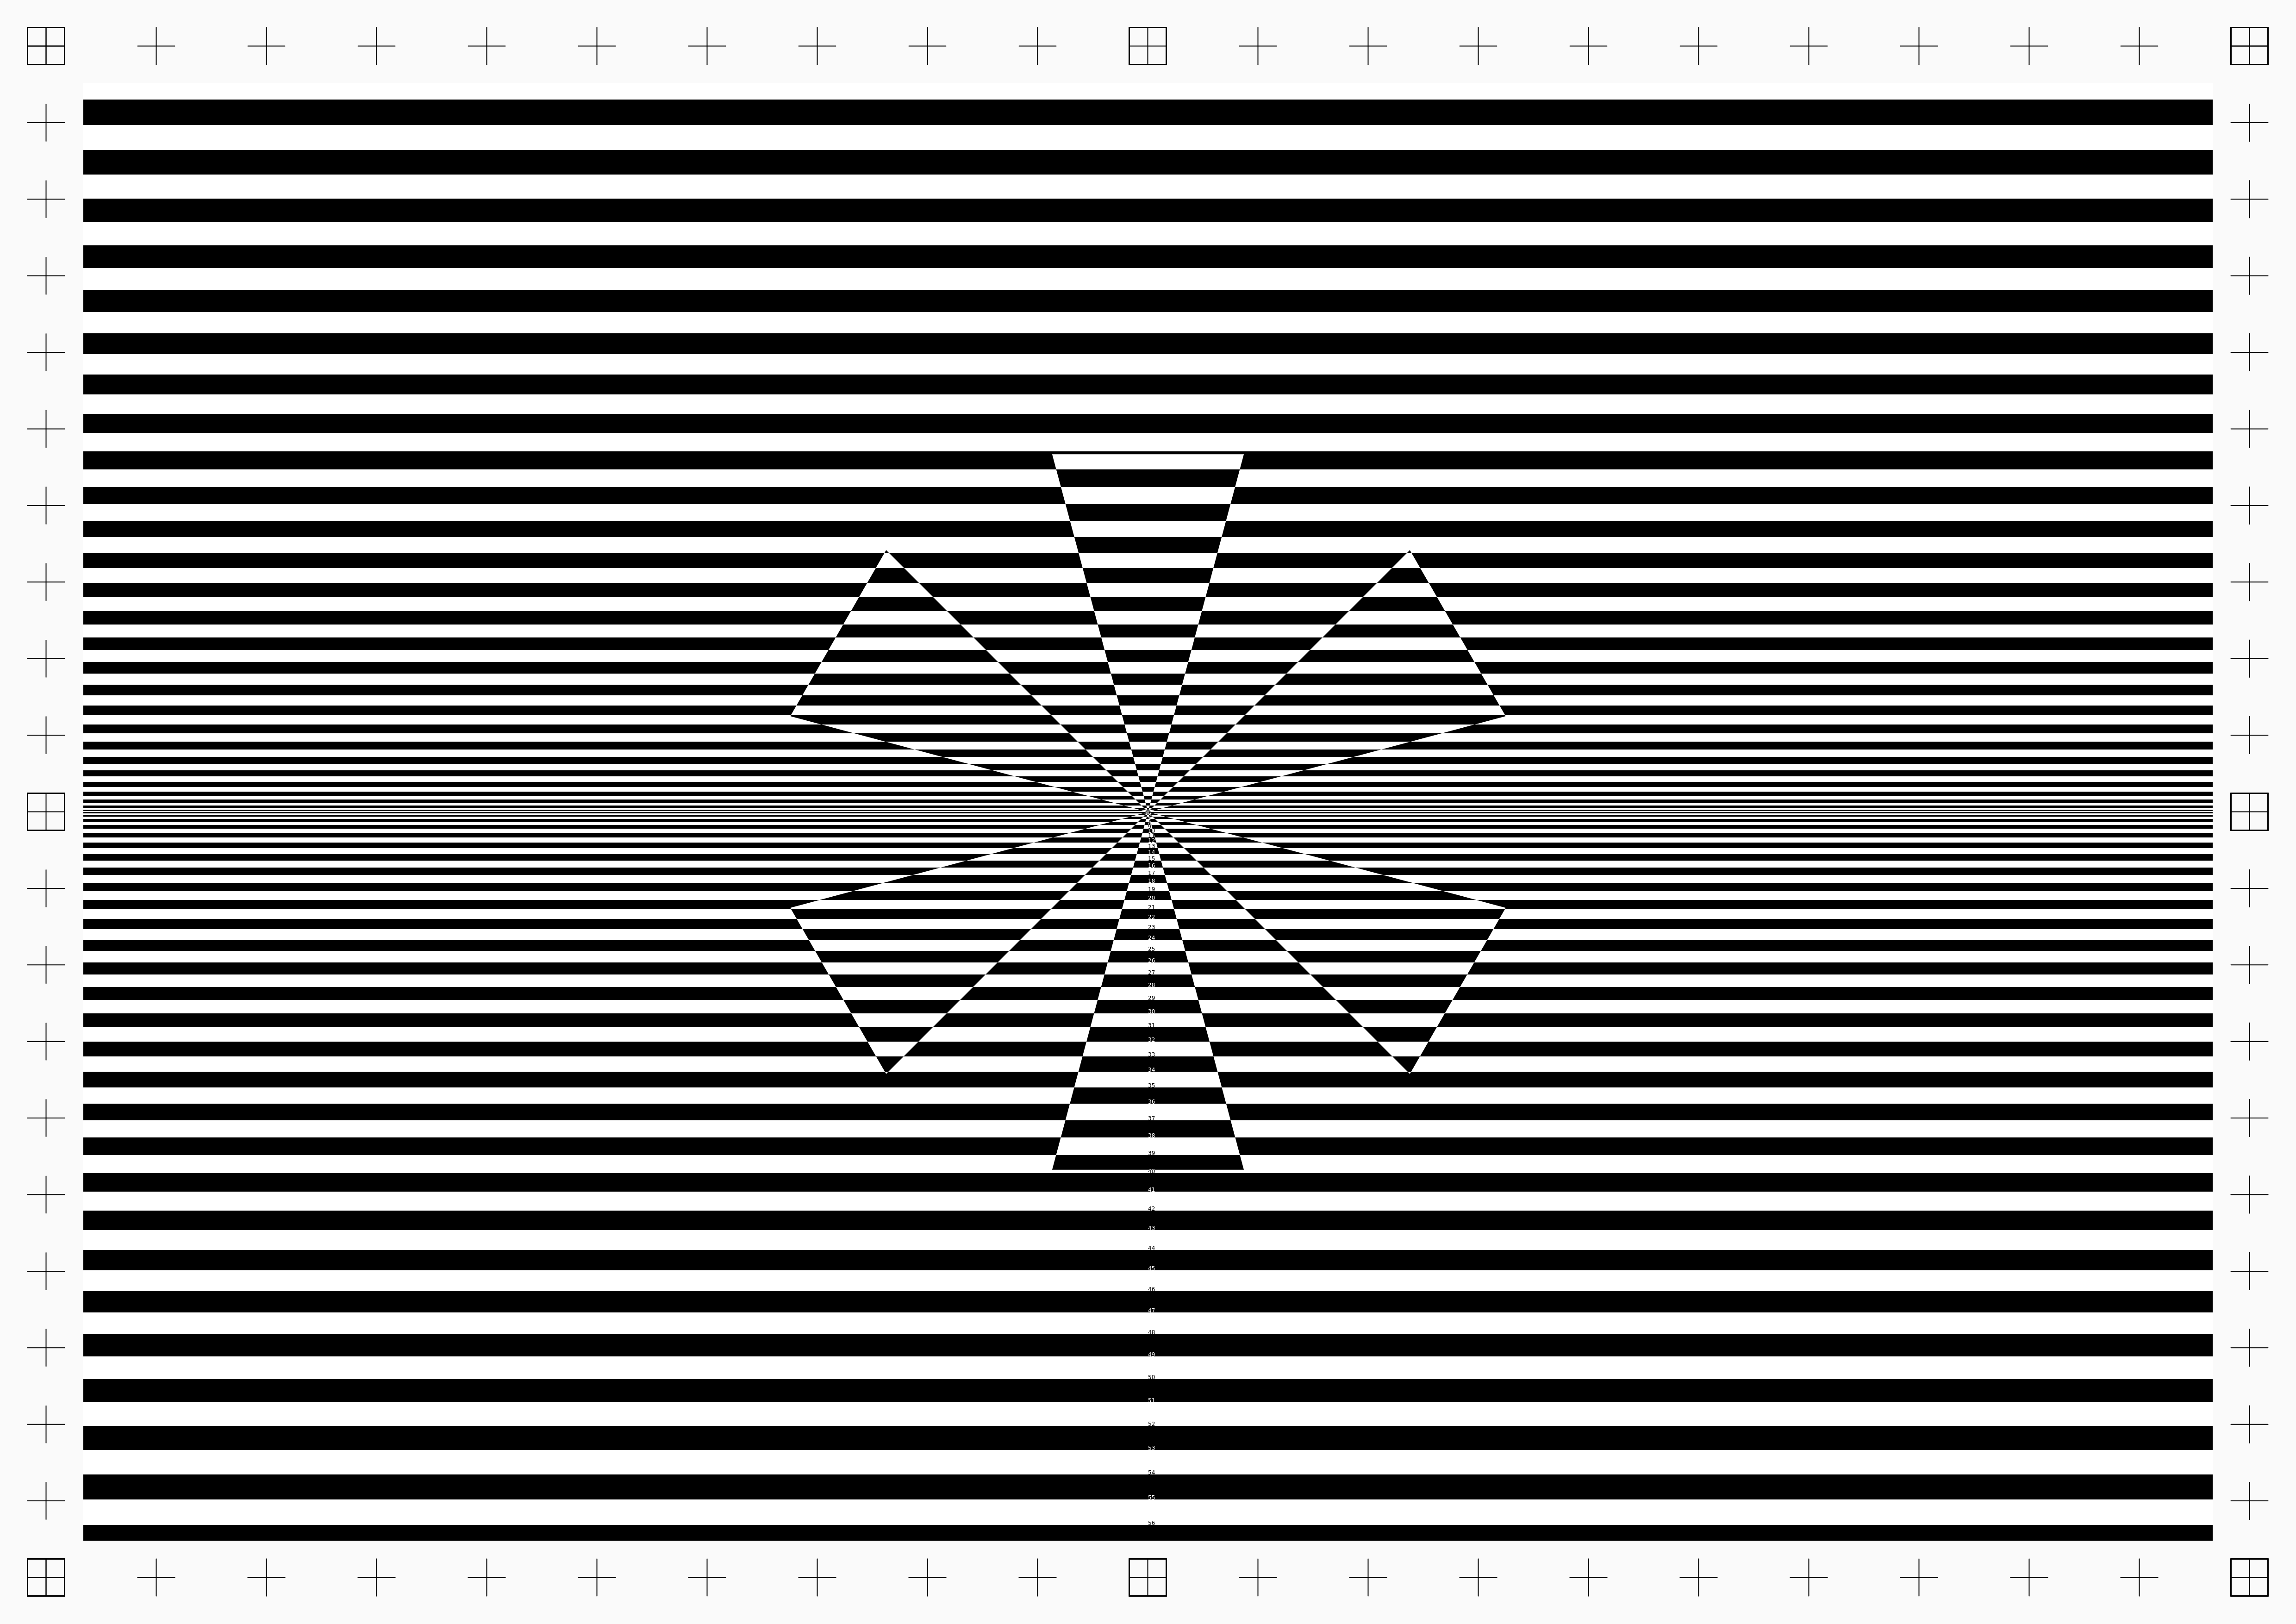
\includegraphics[angle=90,width=0.95\textwidth]{Images/calibration.png}
    \caption{Standardized Vignetting Test Chart}
    \label{fig:vignetting_chart}
\end{figure}

\section{Lines Test Chart}
\label{app:distortion_chart}
\begin{figure}[H]
    \centering
    
\includegraphics[angle=90,width=0.95\textwidth]{Images/grid.png}
    \caption{Standardized Distortion Test Chart}
    \label{fig:distortion_chart}
\end{figure}

Test charts can be found on project's Github in full resolution (which the user is advised to as the resolution is critical for tests).

\chapter{User Manual}
\label{app:user_manual}

\section{Installation}
\begin{enumerate}
    \item Ensure Python 3.8 or higher is installed on your system.
    \item Clone the repository:
    \begin{verbatim}
    git clone https://github.com/yourusername/lens-evaluation-app.git
    \end{verbatim}
    \item Navigate to the project directory:
    \begin{verbatim}
    cd lens-evaluation-app
    \end{verbatim}
    \item Install required dependencies:
    \begin{verbatim}
    pip install -r requirements.txt
    \end{verbatim}
\end{enumerate}

\section{Usage}
\subsection{Launching the Application}
Run the main script to start the web-based interface:
\begin{verbatim}
python app.py
\end{verbatim}
Open your web browser and navigate to \texttt{http://localhost:8080}.

\subsection{Evaluating Lens Properties}
\begin{itemize}
    \item \textbf{Select Evaluation Type}: Choose from Vignetting, Bokeh, Sharpness, Chromatic Aberration, or Distortion.
    \item \textbf{Upload Test Image}: Upload the corresponding test chart image.
    \item \textbf{Start Analysis}: Click on the "Analyze" button to initiate the evaluation.
    \item \textbf{View Results}: The results will be displayed with visualizations and scores.
\end{itemize}
